% Annotated biquad transfer function — showcases LaTeX math typesetting
% (amsmath braces + TikZ colored callouts). Single pdflatex pass.
% Compile: pdflatex biquad-transfer-function-annotated.tex ; dvisvgm --pdf --no-fonts ...
\documentclass[border=10pt]{standalone}
\usepackage{amsmath}
\usepackage{xcolor}
\usepackage{tikz}
\usetikzlibrary{arrows.meta, calc}
\colorlet{ff}{blue!62!black}   % feed-forward / numerator
\colorlet{fb}{red!58!black}    % feedback / denominator
\begin{document}
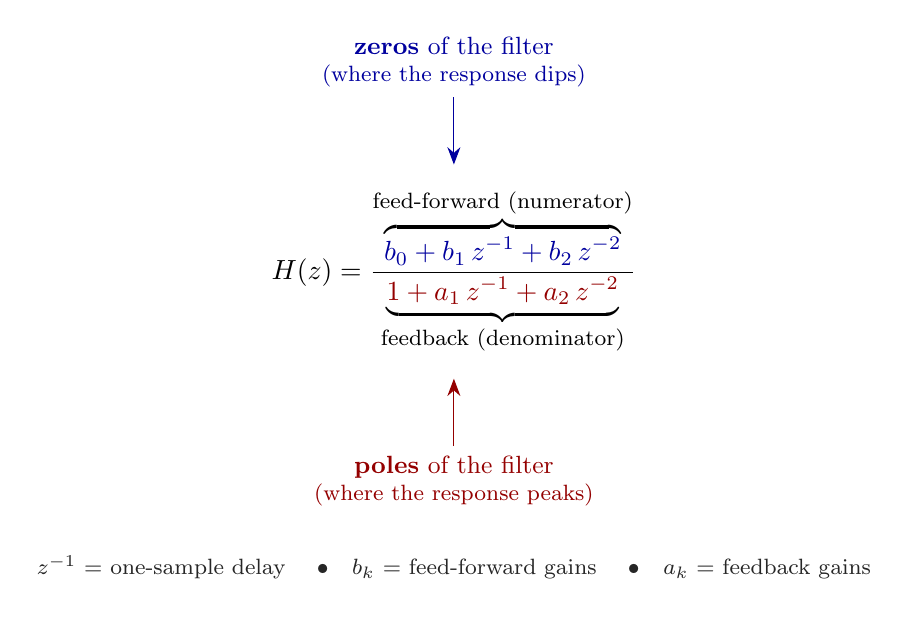
\begin{tikzpicture}[>={Stealth[length=2.2mm]}]

  % --- the equation, with structural over/under-braces -----------------------
  \node[inner sep=3pt] (eq) {$\displaystyle
    H(z)=
    \frac{\overbrace{\textcolor{ff}{b_0 + b_1\,z^{-1} + b_2\,z^{-2}}}^{\text{\footnotesize feed-forward (numerator)}}}
         {\underbrace{\textcolor{fb}{1 + a_1\,z^{-1} + a_2\,z^{-2}}}_{\text{\footnotesize feedback (denominator)}}}$};

  % --- interpretive callouts -------------------------------------------------
  \node[ff, font=\small, align=center] (zeros) at ([yshift=15mm]eq.north) {%
    \textbf{zeros} of the filter\\[-1pt]{\footnotesize (where the response dips)}};
  \draw[ff, ->] (zeros.south) -- ([yshift=2mm]eq.north);

  \node[fb, font=\small, align=center] (poles) at ([yshift=-15mm]eq.south) {%
    \textbf{poles} of the filter\\[-1pt]{\footnotesize (where the response peaks)}};
  \draw[fb, ->] (poles.north) -- ([yshift=-2mm]eq.south);

  % --- symbol legend (variable names spelled out alongside symbols) ----------
  \node[font=\footnotesize, align=center, gray!30!black] at ([yshift=-26mm]eq.south) {%
    $z^{-1}$ = one-sample delay \quad$\bullet$\quad
    $b_k$ = feed-forward gains \quad$\bullet$\quad
    $a_k$ = feedback gains};

\end{tikzpicture}
\end{document}
